\documentclass[11pt,a4paper]{article}
\usepackage{CJKutf8}

%\usepackage[T1]{fontenc}
\usepackage[utf8]{inputenc}
\usepackage{fancyhdr}

\usepackage{amsmath} \usepackage{balance} \usepackage{setspace}
\usepackage[title,titletoc,toc]{appendix} \usepackage{url}
\usepackage{graphicx} \usepackage{wrapfig} \usepackage{subcaption}
\graphicspath{ {images/} }
% \usepackage[backend=biber, style=phys,]{biblatex}
\usepackage{tabu}
\usepackage[figurewithin=section,compatibility=false,justification=justified,listformat=simple,format=plain,labelformat=simple,labelsep=period]{caption}
\usepackage[top=1.4in,bottom=1.6in,left=1.in,right=1in]{geometry}
\usepackage{indentfirst}
% \addbibresource{elex.bib}

\usepackage{wrapfig}
\setlength{\parindent}{22pt} 
\setlength{\parskip}{.5em} 
\usepackage{hyperref}
\usepackage{xcolor}
\hypersetup{
	colorlinks,
	linkcolor={red!50!black},
	citecolor={blue!50!black},
	urlcolor={blue!80!black}
}


\renewcommand{\abstractname}{摘要} 
\renewcommand{\figurename}{图}
\renewcommand{\tablename}{表} 
\title{近代物理实验(I):晶体光学性质测分析}

\author{胡乃超$^1$ \hspace{1cm}  金谷柳新$^2$\\
\footnotesize{ $^1$ 物理科学与工程技术学院, 物理学系$2013$级, $12309011$} \\
\footnotesize{ $^2$ 物理科学与工程技术学院, 物理学系$2013$级, $13345012$}}
 
% \author{金谷柳新$^1$ \hspace{1cm}  胡乃超$^2$\\
% \footnotesize{ $^1$ 物理科学与工程技术学院, 物理学系$2013$级, $13345012$} \\
% \footnotesize{ $^2$ 物理科学与工程技术学院, 物理学系$2013$级, $12309011$}}
  
\date{}

\makeatletter\@addtoreset{section}{part}\makeatother%

\begin{document}
\begin{spacing}{1.3}
\begin{CJK*}{UTF8}{gbsn}
\maketitle
    %\begin{abstract}
    %OMG 图终于正常了我好感动。XD
    %  啦啦啦啦啦啦啦啦啦啦啦啦啦啦啦啦啦啦啦啦啦啦啦啦啦啦啦啦啦啦啦啦啦啦啦啦啦啦啦啦啦啦啦啦啦啦啦啦啦啦啦
    %  啦啦啦啦啦啦啦啦啦啦啦啦啦啦啦啦啦啦啦啦啦啦啦啦啦啦啦啦啦
    %  啦啦啦啦啦啦啦啦啦啦啦啦啦啦啦啦啦啦啦啦啦啦啦啦啦啦啦啦啦啦啦啦啦啦啦啦啦啦啦啦
    %  啦啦啦啦啦啦啦啦啦啦啦啦啦啦啦啦啦啦啦啦啦啦啦啦啦啦啦啦啦啦啦啦啦啦啦啦啦啦啦啦
    %  啦啦啦啦啦啦啦啦啦啦啦啦啦啦啦啦啦啦啦啦啦啦啦啦啦啦啦啦啦啦啦啦啦啦啦啦啦啦啦啦\par
    %\textbf{关键词:}
    %\end{abstract}    
\section{引言}
在晶体中,除立方晶系晶体外,都表现出光学各向异性(双折射现象)。当光经过各向异性晶体时,
光的性质会随着晶体的取向不同而发生改变,并表现出各种有趣的光学现象。利用晶体的各向异性,
可以制成光学偏振器,应用分析器,电光调制器等。观测和研究晶体的光学性质,对我们充分认识晶
体的光学性质有十分重要的意义。
\section{实验目的}
\begin{enumerate}
\item 	熟悉单轴晶体光学性质,晶体的消光现象,干涉色级序;
\item   了解偏光显微镜原理并掌握其使用方法;
\item   观察晶体的类别,轴向和光性正负等过程,估计晶片的光程差。
\end{enumerate}

\section{实验原理}
\subsection{晶体的双折射和光率体}
折射率与光的传播方向和光矢振动方向有关的晶体称为各向异性晶体。除立方晶系的晶体外,
所有的晶体都是各向异性晶体。\par
当光通过各向异性晶体时,会产生双折射现象,并表现出偏振性质。当光沿各向异性晶体传播时,
总存在一个或两个方向不发生双折射现象,此方向称为晶体的光轴,按晶体的光轴分,
各向异性晶体又可分为单轴晶和双轴晶,单轴晶只有一个光轴;而双轴晶则有两个光轴。其中,
折射率不随入射光方向而变的称为寻常光或$o$光(折射率为$n_o$),折射率随入射光方向而变
的称为非寻常光或$e$光(折射率为$n_e$)。
$o$光和$e$光都是偏振光,并且它们的振动方向互相垂直。$o$光的振动方向垂直于包含光轴和$o$
光波法线所组成的平面,$e$光的振动方向则平行于包含光轴和$e$光波法线所组成的平面。\par
折射率椭球(或光率体)是描述晶体光学性质最常用的晶体光学示性曲面,它是以主折射率为主
值的椭球。在主轴坐标系,折射率椭球可以表示为:
\begin{equation}
\frac{X_1^2}{n_1^2}+\frac{X_2^2}{n_2^2}+\frac{X_3^2}{n_3^2}=1.\label{4-1-1}
\end{equation} 
\subsubsection{立方晶系(高级晶族)}
\begin{equation}
n_1=n_2=n_3=n_0,
\end{equation}
\begin{equation}
\frac{X^2_1+X^2_2+X^2_3}{n_0^2}=1.
\end{equation}
\subsubsection{单轴晶(中级晶族)}
\begin{equation}
n_1=n_2=n_0,\ n_3=n_e,
\end{equation}
\begin{equation}
\frac{X^2_1+X^2_2}{n_0^2}+\frac{X^2_3}{n_e^2}=1.
\end{equation}

\begin{figure}
\centering
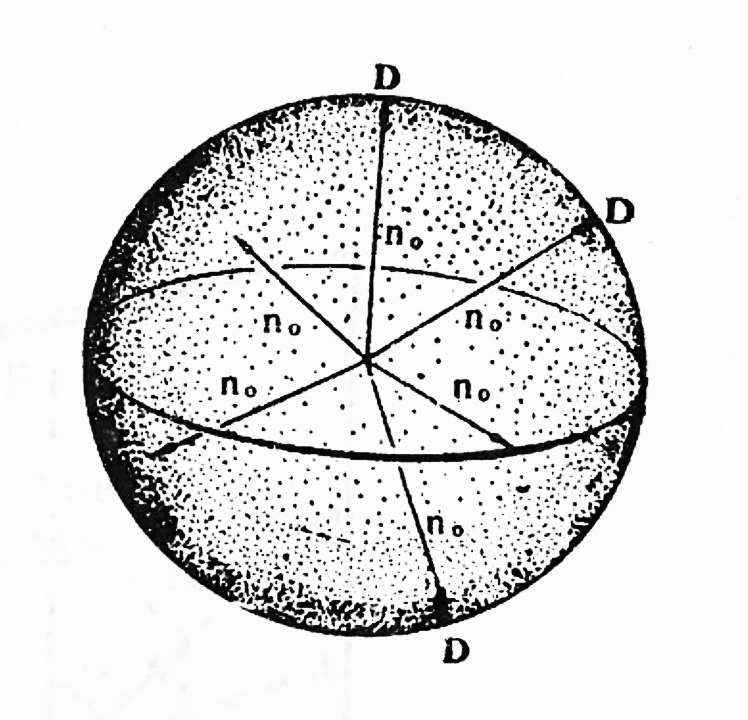
\includegraphics[width=0.4\textwidth]{fig4-1-1}
\caption{立方晶系晶体光率体图}
\label{fig:4-1-1}
\end{figure}
单轴晶光率体的光轴($x_3$),必须与晶体中的主对称轴(唯一的高次轴)一致。$n_e>n_0$的单轴晶称
为正光性单轴晶,它的光率体是沿光轴方向拉长了的旋转椭球(图~\ref{fig:4-1-2}(a)),$n_e<n_0$的单轴
晶称为负光性单轴晶,它的光率体是沿光轴方向压扁了的旋转椭球(图~\ref{fig:4-1-2}(b))。
由于光速$v=c/n$,折射率越大,其光速越慢,所以在晶体中,折射率最大的方向成为晶体慢轴方向,
而折射率最小的方向成为晶体快轴方向。\par
\begin{figure}
\centering
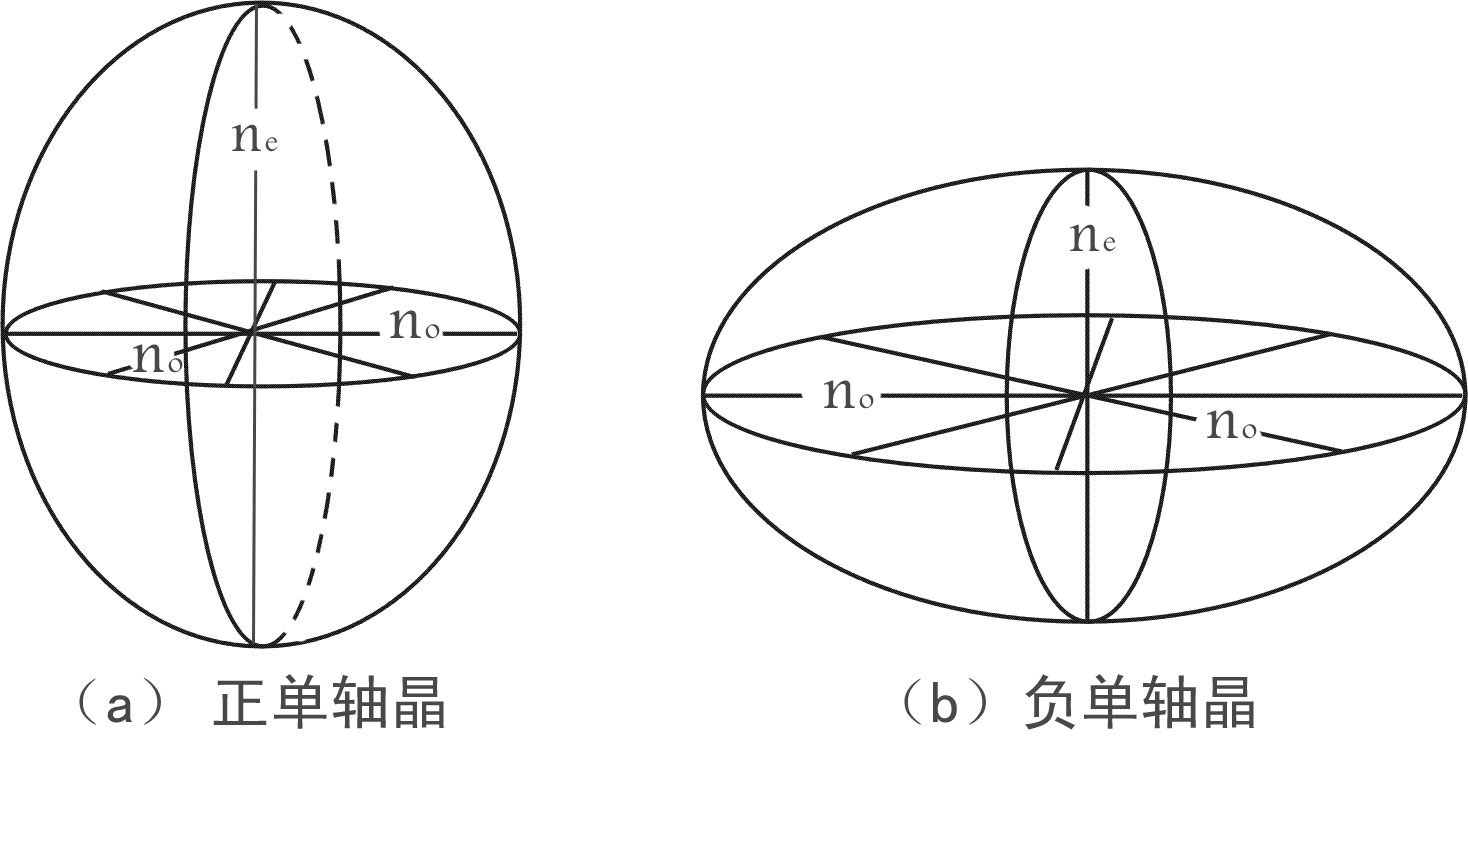
\includegraphics[width=0.7\textwidth]{fig4-1-2}
\caption{单轴晶光率体图}
\label{fig:4-1-2}
\end{figure}
图~\ref{fig:4-1-3}给出了单轴晶光率体中三种中心截面。圆截面:垂直光轴的圆,半径为$n_0$。
主截面:包含光轴的椭圆截面,它的一个半径为$n_0$,与光轴垂直,另一个半径为$n_e$,与光轴平行。
由图可见:$o$光的振动方向必垂直于主截面,$e$光的振动方向则平行于主截面。
任意截面:是一个椭圆,截面法线$N$与光轴成$\theta$角。
\begin{figure}
\centering
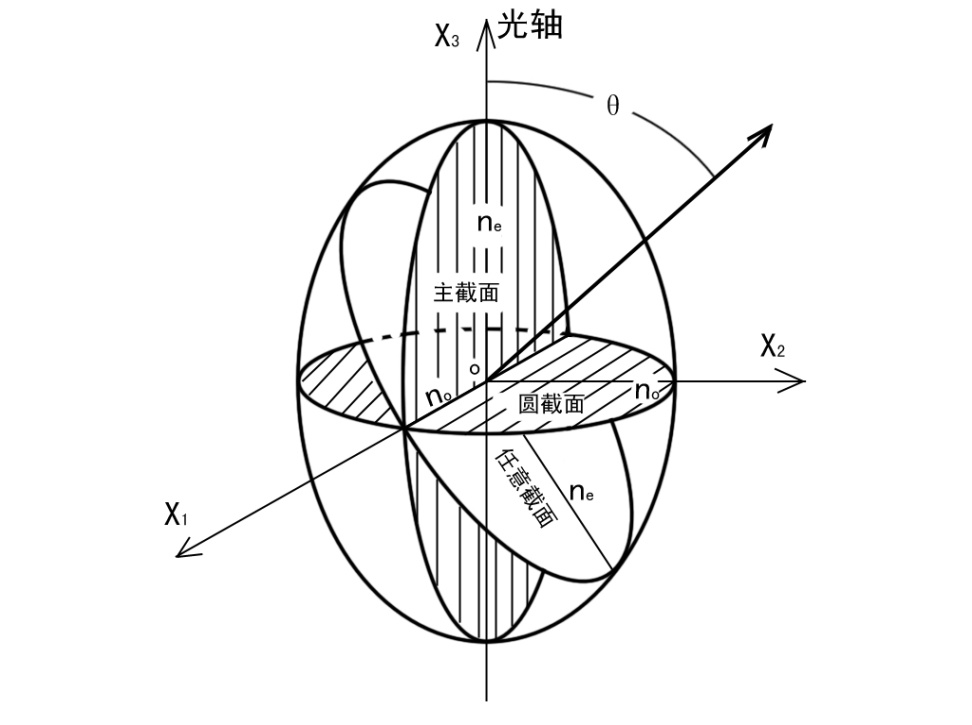
\includegraphics[width=0.5\textwidth]{fig4-1-3}
\caption{单轴晶光率体的三种中心截面}
\label{fig:4-1-3}
\end{figure}
\subsubsection{双轴晶(低级晶族)}
\begin{equation}
n_1\neq n_2\neq n_3,
\end{equation}
\begin{equation}
\frac{X_1^2}{n_1^2}+\frac{X_2^2}{n_2^2}+\frac{X_3^2}{n_3^2}=1.\label{4-1-4}
\end{equation} 
在低级晶族光率体中,可以找到两个圆截面,即存在两个光轴。双轴晶的光学性质比较复杂,这里不作详
细讨论,以下分析讨论都是单轴晶情况。

\subsection{正交偏光干涉}
在偏光显微镜中,当上下偏光镜的振动面互相垂直时,称为正交偏光镜。如在正交偏光镜间不放任和介质
或放入各相同晶体时,光线无法通过正交偏光镜,所以视阈是黑暗的;当在正交偏光镜间放入各相异晶体
时,由于晶体双折射效应和晶片厚度、晶轴取向的不同而产生不同的干涉现象。
\begin{figure}
\centering
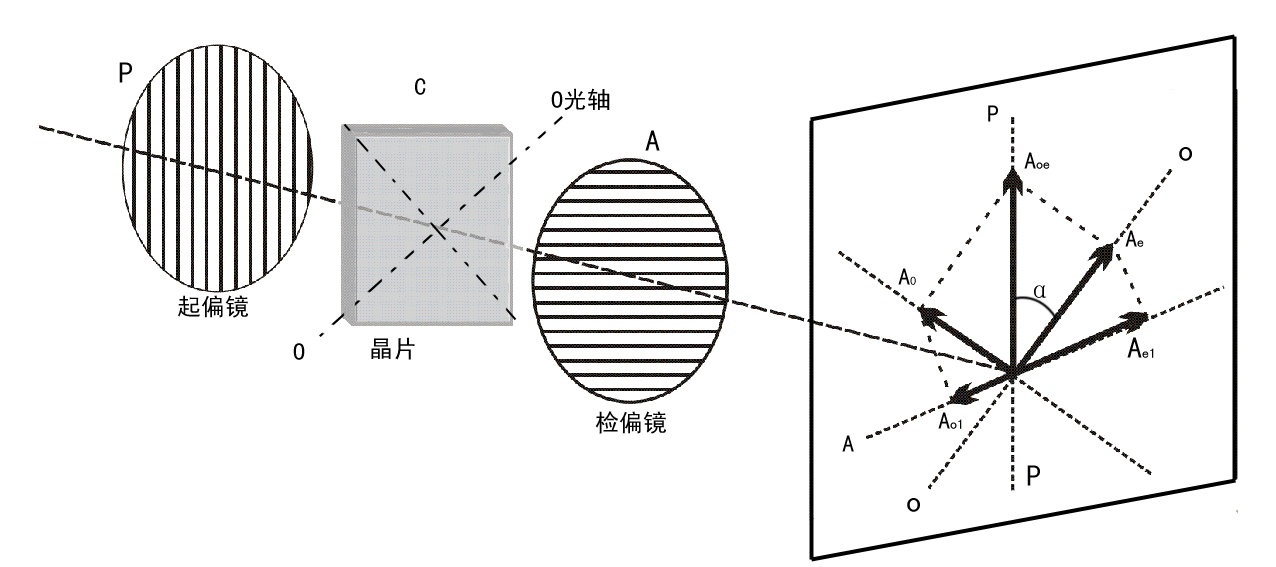
\includegraphics[width=0.9\textwidth]{fig4-1-4}
\caption{正交偏光镜间的干涉现象}
\label{fig:4-1-4}
\end{figure}
如图~\ref{fig:4-1-4},在正交偏光镜中加入一晶片,其中$PP$表示起偏镜的振动方向,$AA$表示检偏镜
的振动方向,$OO$表示晶片光轴方向。透过起偏镜的偏振光振幅为$A_{oe}$,光线到达厚度为$d$的晶片后,
分解成振幅分别为$A_e$和$A_o$的$e$光和$o$光:$A_e=A_{oe}\cos\alpha,\,A_o=A_{oe}\sin\alpha$。再经
过检偏镜后,$e$光和$o$光振幅分别变为:$A_{e1}=A_e\sin\alpha=A_{oe}\cos\alpha\sin\alpha,\,
A_{o1}=A_o\cos\alpha=A_{oe}\sin\alpha\cos\alpha$。
由于各向异性晶体的双折射率,两种光透过厚度为$d$的晶片时,必产生光程差:$\Delta=d(n_e-n_o)$或
相位差:$\delta=2\pi d(n_e-n_o)/\lambda$。由此可见,经过正交偏振片和晶片后产生的两束光满足相
干条件:1)频率相同,2)相位差恒定,3)有相同方向的偏振分量,必然产生干涉。根据平面波迭加原理,
两束光的合成光波振幅:
\begin{equation}
A_+^2=A_{e1}^2+A_{o1}^2-2A_{e1}A_{o1}\cos\delta=A_{oe}^2\sin^22\alpha\sin^2\big[\frac{d(n_e-n_o)}{\lambda}\pi\big],
\end{equation}
其合成光强:
\begin{equation}
I\propto A_+^2= A_{oe}^2\sin^22\alpha\sin^2\big[\frac{d(n_e-n_o)}{\lambda}\pi\big].\label{eq:4-1-6}
\end{equation}
由式~\eqref{eq:4-1-6}可看出:正交偏光干涉光强分布状况与晶片的轴向$\alpha$,厚度$d$,双折射率$\Delta n$
及入射波长$\lambda$有关。
\subsubsection{单色光干涉}
对于单色光,当$\alpha=0,\pi/2,\pi,\ldots$时,$sin2\alpha=0$,即当晶片的轴向与两正交偏光镜其中之一
的偏振方向一致时,合成光强为零,视野全暗,此现象称为消光现象。此时,晶片的位置称为消光位置。当
$\alpha=\pi/4,3\pi/4,5\pi/4,\ldots$时,$sin2\alpha=\pm 1$,即当晶片的轴向处于两个偏光镜的偏振方向
中间时,合成光强最大,视阈最亮。很显然,如转动晶片$360$度,会出现四暗、四明现象。\par

当晶片的双折射率$\Delta n$不变,厚度变化,这相当于石英锲子的情况。石英锲子是一个磨成一端薄一端厚的
石英晶片,长边平行于$n_o$,短边平行于$n_e$,双折射率$\Delta n=0.009$。
当正交偏光镜中插入的是石英锲子,由于石英锲子厚度不同,其不同厚度出的光程差$\Delta=d(n_e-n_o)$
也不相同,所以当石英锲子由薄至厚插入时,就会观察到有规律的明暗相间的干涉条纹。
如图~\ref{fig:4-1-5}所示。
\begin{figure}[htbp]
\begin{subfigure}[b]{0.5\textwidth}
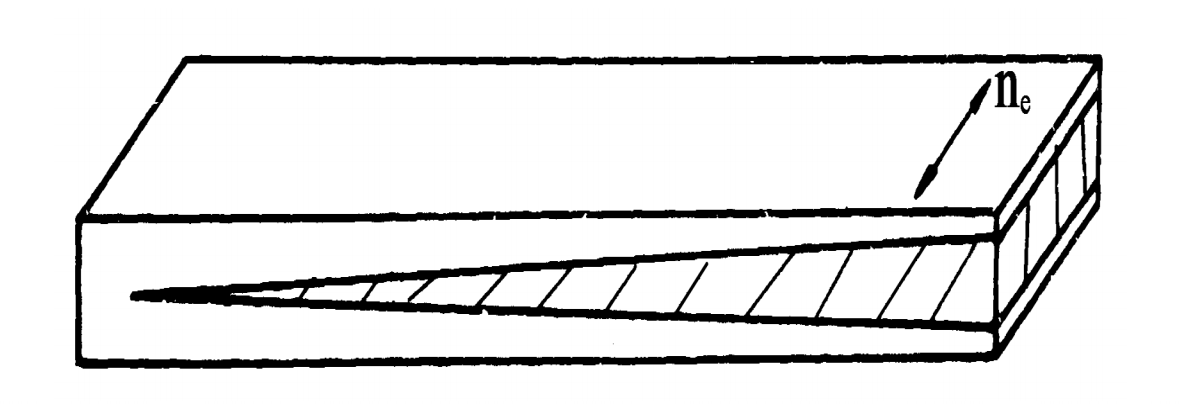
\includegraphics[width=\linewidth]{fig4-1-5a}
\caption{石英楔子}
\label{fig:4-1-5a}
\end{subfigure}
\begin{subfigure}[b]{0.49\textwidth}
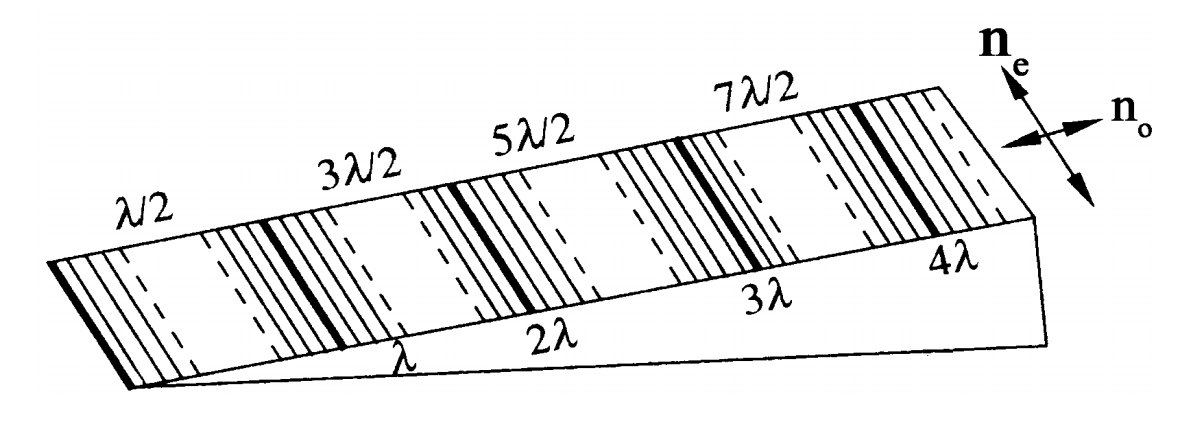
\includegraphics[width=\linewidth]{fig4-1-5b}
\caption{石英楔子干涉条纹}
\label{fig:4-1-5b}
\end{subfigure}
\caption{正交偏光下石英楔子干涉}\label{fig:4-1-5}
\end{figure} 
\subsubsection{白光干涉}
用白光照明时,由于白光是由红橙黄绿蓝靛紫七色组成,且各色光波长范围不同,所以对于某一个$d$值,
不同色的光不可能同时达到相消或相长,干涉条纹也就不再是明暗不同的条纹,而只能是由光强不为零的
各种单色光混合组合而成的,称为干涉色。\par
当晶片的双折射率$\Delta n$不变,厚度变化,如石英锲子情况,其折射率随光波变化很小,可看作基本
不变。当正交偏光镜中插入的是石英锲子,随着石英锲子厚度得变化其颜色发生有规律的变化,就是干涉
色级序,大约每$560nm$光程差划分一个干涉色级序,通常可分为四个级序,光程差越大则干涉色级序越高
。每个干涉色级序中,颜色的一次明显改变称为一个色序,各色序之间颜色是连续变化的。对于同一石英
锲子,波长越短,其明暗条纹间距亦越短。
\begin{figure}
\centering
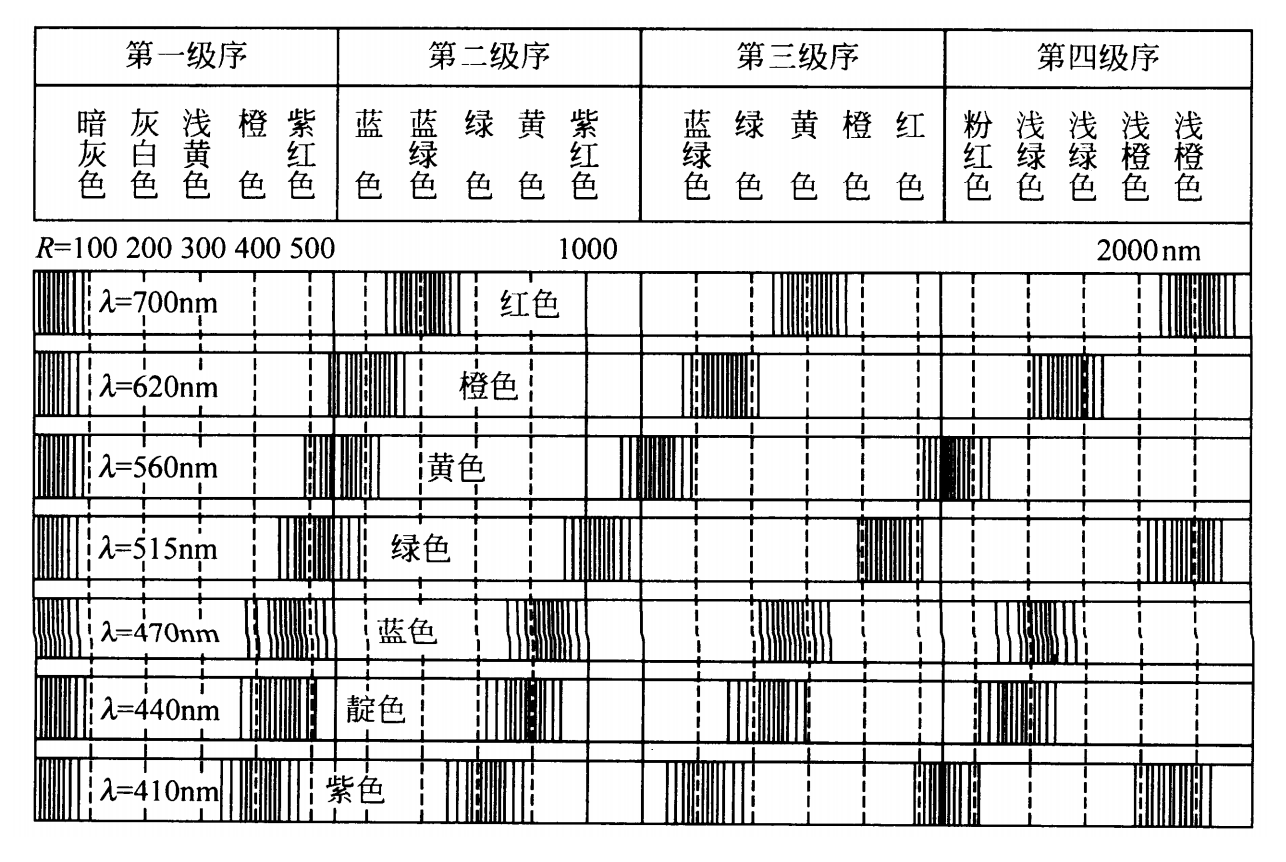
\includegraphics[width=0.9\textwidth]{fig4-1-6}
\caption{正交偏光镜下不同波长的单色光透过石英楔子产生的干涉条带}
\label{fig:4-1-6}
\end{figure}

\subsubsection{光程差补偿原理}
如果在正交偏光镜间放两块晶片,设光线通过晶片$1$和晶片$2$的光程差分别为$\Delta_1$和$\Delta_2$,
当两晶片同名轴(快慢轴)平行时,如图~\ref{fig:4-1-7a}所示,则通过两晶片的总光程差
$\Delta=\Delta_1+\Delta_2$,其干涉色比原来两晶片单独放入时的干涉色都高;当两晶片异名轴平行时,
如图~\ref{fig:4-1-7b}所示,则通过两晶片的总光程差$\Delta=\Delta_1+\Delta_2$,
其干涉色比其中之一单独放入时的干涉色低。若两晶片的光程差相等,则$\Delta=\Delta_1-\Delta_2=0$,
此时两晶片的光程差互相补偿,视阈全暗。上述光程差叠加和补偿的规律称为补色法则。

\begin{figure}[htbp]
\begin{subfigure}[b]{0.4\textwidth}
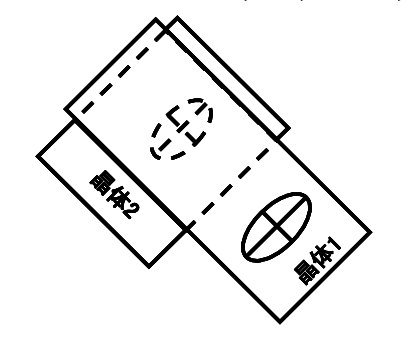
\includegraphics[width=\linewidth]{fig4-1-7a}
\caption{同名轴平行}
\label{fig:4-1-7a}
\end{subfigure}
\begin{subfigure}[b]{0.4\textwidth}
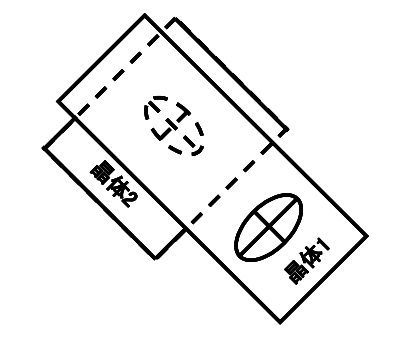
\includegraphics[width=\linewidth]{fig4-1-7b}
\caption{异名轴平行}
\label{fig:4-1-7b}
\end{subfigure}
\caption{上下两晶片同名轴位置关系示意图}\label{fig:4-1-7}
\end{figure} 
若将晶片$2$换成石英锲子,且慢慢推入石英锲子,使$\Delta_2$逐渐增加。
此时,如果晶片$1$与石英锲子同名轴平行,总光程差$\Delta$是递增的,导致干涉色逐渐升高;
如果晶片$1$与石英锲子异名轴平行,总光程差$\Delta$是递减的,导致干涉色逐渐降低。\par
当两个晶片相叠时,如果一个晶片的快慢轴方向已知,可根据补色法则,利用干涉色升降情况,
确定出另一晶片的快慢轴方向,并可通过查干涉色表估算出另一晶片的光程差。

\subsection{锥光干涉}
对于晶体的轴性、光性符号、光性方位、光轴角等根本问题,则要通过锥光观测才能最后下结论。\par
在正交偏光镜的条件下,在广路中加入聚光镜和勃氏镜便构成了锥光装置。追光装置加入聚光镜可是平行
入射的偏振光高度聚敛,形成锥形偏光;加入勃氏镜可以得到放大了的清晰、完整的干涉图,如不加勃氏镜,
必须拔出目镜,才能看到物镜焦平面上小得多的干涉图。通过锥光装置在视阈中显现的干涉图称为锥光干涉图,
它不是晶片本身的像,而是锥形偏光通过镜片后到达上偏光镜所发生的干涉效应的总和。
下面根据光轴在晶体切片中方位的不同分几种情况讨论。
\subsubsection{垂直光轴切片的晶体干涉}
\begin{figure}
\centering
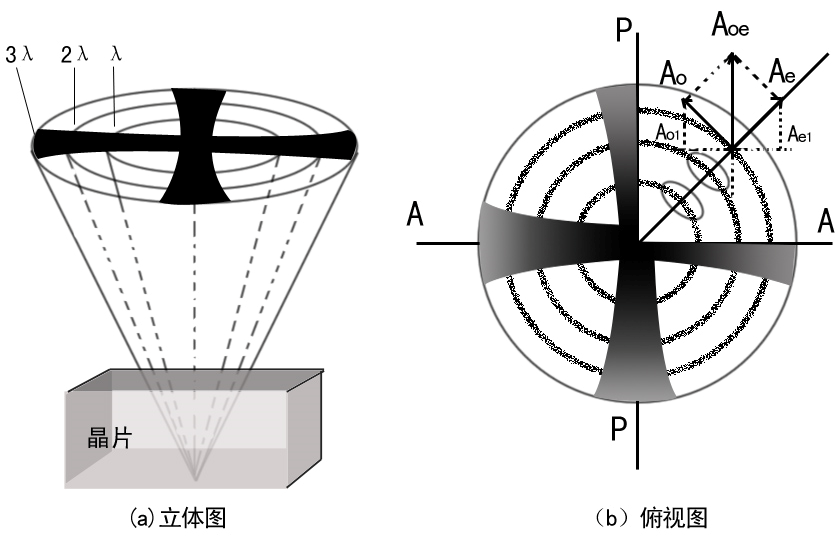
\includegraphics[width=0.8\textwidth]{fig4-1-8}
\caption{单轴晶体垂直光轴切片锥光干涉图}
\label{fig:4-1-8}
\end{figure}
图~\ref{fig:4-1-8}给出了光源为单色光时垂直光轴切片晶体锥光干涉图,它是由一个黑十字和亮暗相间
的同心圆环组成。当光源为白光时,则同心圆环变为干涉彩环。图中十字交点为光轴的露点,近光轴处黑
臂较细,远离光轴处黑臂较粗。自光轴露点向外,等色环由疏变密,干涉色级由低到高,旋转载物台,干
涉色不发生变化。具有高双折射率的晶体所形成的干涉环,要比低双折射率晶体的多。对于同一种晶体,
厚的晶片所形成的干涉环,要比薄的晶片多。此外,所使用物镜的数值孔径越高,则所观察到的干涉环也
越多。\par
在锥光干涉中,光锥中有一系列的光通过晶片,而每一条光在晶片中都有两个互相垂直的振动方向,其折
射率分别为$n_e$和$n_o$。由图~\ref{fig:4-1-8}可知,越到视阈边缘,光线方向对光轴倾斜的越厉害,
双折射率就越大,对应的光率体切面之形状也就越加长而扁。包含在PP(或AA)面内的光与光轴组成的面
是$PP$(或$AA$)面,即主截面,非常光是在$PP$(或$AA$)面内振动,而常光则在垂直$PP$(或$AA$)
面内振动。但由于来自下偏光镜的光都是在$PP$面内振动的线偏光,所以包含在$PP$面内的光会全部从非
常光的振动面内通过,而包含在$AA$面内的光则会全部从常光的振动面内通过,因此通过PP和AA面内的光
在通过晶片后,其偏振方向不会发生改变,都平行于下偏光镜的偏振方向,与上偏光镜的偏振方向垂直,
无法通过上偏光镜,因而在视阈中平行$PP$和$AA$方向就产生一个黑十字消光影。只有位于$PP$和$AA$面
内的光才是绝对消光,而光锥中位于$PP$和$AA$面附近的光,它们都会有极小一部分通过上偏光镜而互相
干涉,但由于人的眼睛感觉不到,所以此时用人眼观察仍然是暗的,所以十字消光影是两条有一定宽度的
黑臂。转动载物台,消光影的位置不发生变动,这是因为不论载物台怎样转动,光锥中总是有部分光位于
$PP$和$AA$面内或其附近,因此消光影总是存在的,并且消光影始终与下偏光镜和上偏光镜的振动面平行。
\par
在单色光中产生的光轴干涉图除了黑十字消光影外,还有互相交替的亮环与暗环。这主要是因为当光上升
到晶片上时,原来平行$PP$方向的振动在晶片中要分解为两互相垂直的振动,由图~\ref{fig:4-1-8}可知
,非常光总是在入射光与光轴组成的主截面内振动,而常光则在与之垂直的面内振动。当入射光与光轴斜
交越大时,光在晶片中走过的距离越长,双折射率越大,所以从光锥的轴越向外去,光程差就越大。与光
轴成某一角度的光线组成一个光锥,而同一光锥内的每一条光线均与光轴成相同的角度,通过晶片后产生
相同的光程差$\Delta$。如果$\Delta=(n+1/2)\lambda$,光程差是光波长的奇数倍,就会出现干涉相长,
观察到一个亮环。仔细观察会发现在同一亮环上亮度是不均匀的,这是由于在同一环上光的振动方向是变
化的,如图~\ref{fig:4-1-8}所示越靠近消光影处,与$PP$(或$AA$)夹角越小,因此亮度越暗,而在每
一象限的$45^{\circ}$位置,亮环的亮度最大。\par
如用白色光源,仍可观察到黑十字状消光影,所不同的是原来交替出现的亮环与暗环,变成了交替出现的
彩环。靠近视阈的中央是一级灰色,然后是一级黄环,红环,二级紫环,蓝环等,越向视阈的边缘,干涉
色的级数越高,等色曲线的数目越多,密度越大。\par
\begin{figure}
\centering
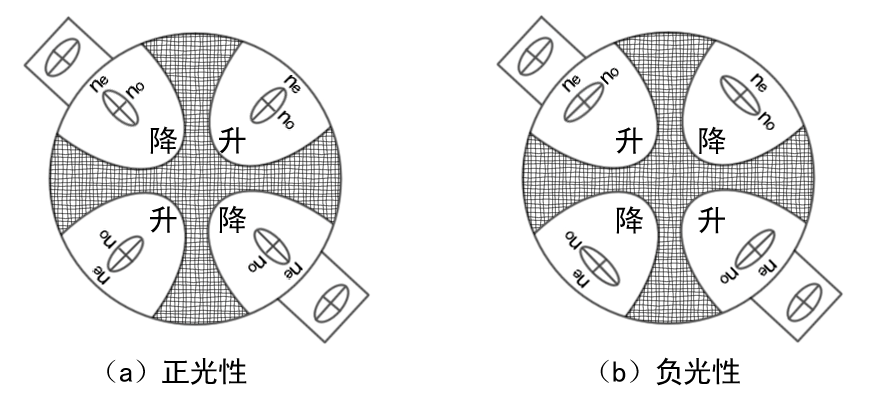
\includegraphics[width=0.8\textwidth]{fig4-1-9}
\caption{单轴晶体光性正负的测定}
\label{fig:4-1-9}
\end{figure}
在实际晶体光学检测中,我们可以利用垂直光轴切片的锥光干涉图来检测和判断晶体光性正负。在垂直光
轴切片的锥光干涉图上,$o$光和$e$光的振动方向如图~\ref{fig:4-1-9}所示。此时插入试板,观察干涉
图中四个象限内干涉色序的升降,根据消光原理判断ne是快轴还是慢轴,从而确定代测样品的光性正负。
另一种判定的方法是:插入试板,观察四个象限干涉彩环的移动方向,或哪两个对称象限在靠近黑十字交
点附近出现黑点,例如,插入石英锲子,如果一、三象限干涉色序升高,二、四象限干涉色序降低,或者
一、三象限干涉彩环向内收缩,二、四象限干涉彩环向外扩张,或者二、四象限在靠近黑十字交点附近出
现黑点,而一、三象限在对应位置上没有黑点,则待测样品为正光性;反之,待测样品为负光性。
\subsubsection{平行光轴切片的晶体干涉}

\begin{figure}
\begin{subfigure}[b]{0.45\textwidth}
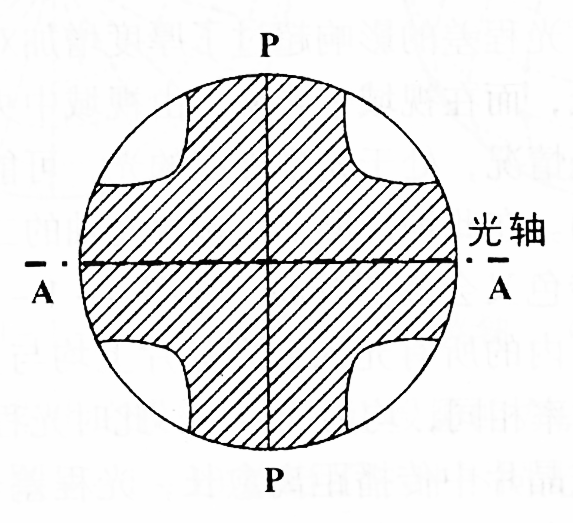
\includegraphics[width=\linewidth]{fig4-1-10a}
\caption{$0^{\circ}$位置}
\label{fig:4-1-10a}
\end{subfigure}
\begin{subfigure}[b]{0.45\textwidth}
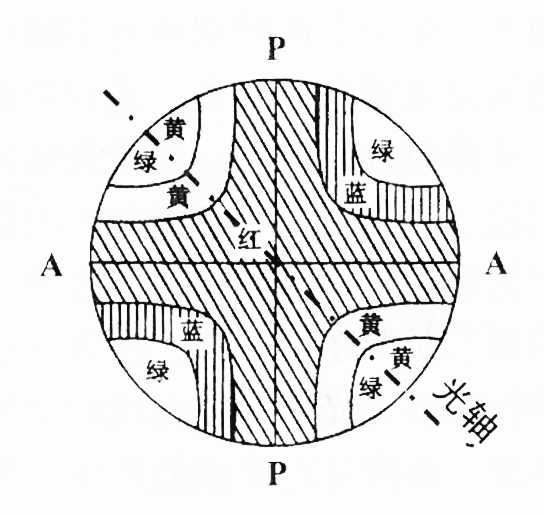
\includegraphics[width=\linewidth]{fig4-1-10b}
\caption{$45^{\circ}$位置}
\label{fig:4-1-10b}
\end{subfigure}
\caption{单轴晶体平行光轴切片锥光干涉图}\label{fig:my_label}
\end{figure} 

对于平行光轴的切片,当光轴与上偏光镜(或下偏光镜)振动方向平行时,视域中出现模糊粗大的黑十字
,只有在四象限中接近边缘有小部分明亮,此时稍微转动载物台,黑十字立即分裂成一对双曲线,并迅速
沿光轴方向离开视域,因其变化迅速,又称为瞬变干涉图。自二相对的象限离开视域就是包含光轴的象限
。继续转动载物台,当光轴与上下偏光镜振动方向成$45^{\circ}$角,视域最亮,出现对称的双曲干涉带
,其干涉色是由光程差所决定的,因而不同的样品其干涉图不尽相同。对于双折射率较高的晶体,当处于
$45^{\circ}$位置时,视域中出现干涉色,在两两相对的象限中,干涉色由视域中心向边缘逐渐升高,据
此可以判断光轴的位置。对于双折射率较低的晶体,当处于$45^{\circ}$位置时,视域中呈现一片白色或
一片灰色,上述干涉色升高和降低现象不明显,此时如插入一石膏试板,现象会清楚很多。\par
\subsubsection{斜交光轴切片的晶体干涉}
在实际晶体分析中,恰巧与光轴垂直或平行的切面极为少见,大部分切面和光轴成各种角度的斜交,斜交
程度可从正交偏光镜间切面的干涉色加以估计。如果切面的干涉色很低,表示切面与光轴接近垂直,如果
切面的干涉色很高,则说明切面与光轴接近平行。假如切面的干涉色不很高也不很低,则切面和光轴斜交
为$45^{\circ}$左右。斜交光轴的切面在聚敛偏光镜间,干涉图的形态往往是不对称的,黑十字的交点即
光轴点不在视域中心,但仍在视域之内,转动载物台,光轴露点也随之转动,方向与载物台的转动方向相
同,随着光轴露点移动,消光影的位置也跟着转移。但不论怎样转移,消光影的两臂仍保持与下偏光镜或
上偏光镜的振动面相平行。当载物台旋转$360^{\circ}$,光轴绕显微镜轴旋转,在空间画出一个锥体,而
光轴在视野中的出露点画出一个圆。当切面与光轴斜交角度角较小时,光轴露出可能不在视野之内,此时
,适当旋转载物台,可观察到一条黑色条带。如果切面与光轴斜交角越来越小,消光影的黑臂就变弯曲起
来,最后当切面与光轴平行时,就变为瞬变干涉图了。
%\subsubsection{垂直光轴切片的晶体干涉}
\begin{figure}
\centering
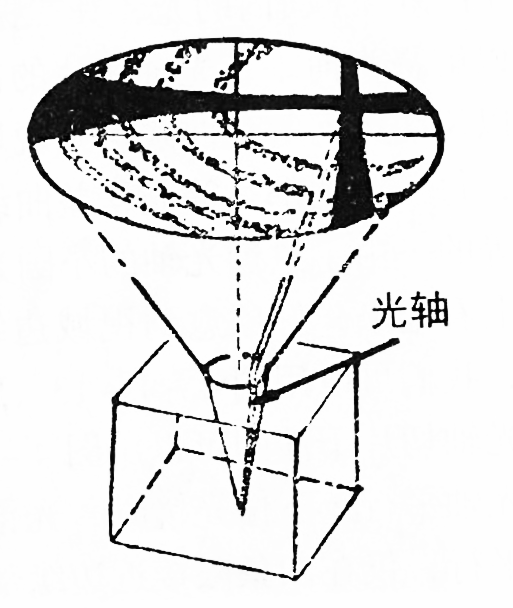
\includegraphics[width=0.4\textwidth]{fig4-1-12}
\caption{斜交光轴切片晶体干涉}
\label{fig:4-1-12}
\end{figure}

\begin{figure}[h!]
\begin{subfigure}[b]{0.5\textwidth}
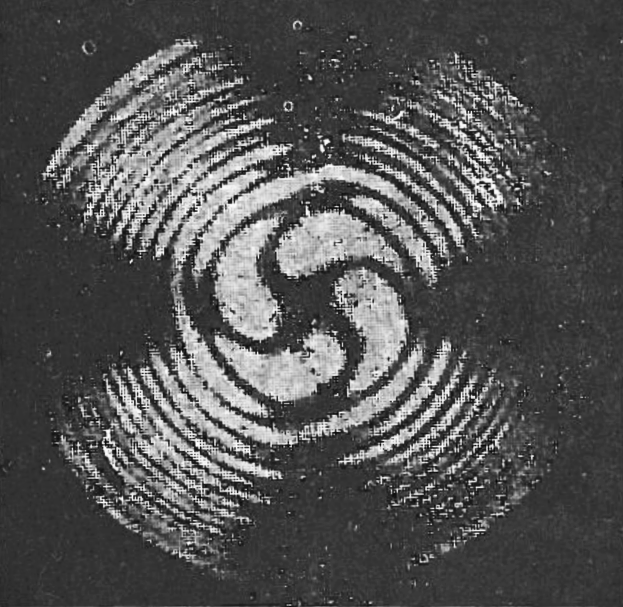
\includegraphics[width=\linewidth]{fig4-1-14a}
\caption{右旋石英在左旋石英之下}
\label{fig:4-1-14a}
\end{subfigure}
\begin{subfigure}[b]{0.49\textwidth}
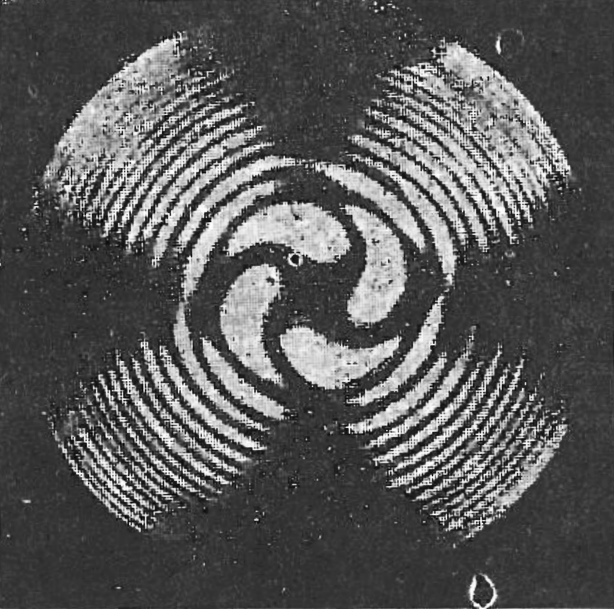
\includegraphics[width=\linewidth]{fig4-1-14b}
\caption{左旋石英在右旋石英之下}
\label{fig:4-1-14b}
\end{subfigure}
\caption{埃利旋}\label{fig:4-1-14}
\end{figure} 
\subsection{晶体旋光性、埃利旋}
当一束线偏振光通过某些物质后,光的振动方向会随着物质中的传播距离增加而逐渐发生旋转,这种现象
称为旋光现象。旋光有左右旋之分,旋光物质也有左旋物质和右旋物质之分。\par
对于旋光物质而言,振动面旋转的角度$\Psi$与通过旋光物质厚度$d$成正比,即
\begin{equation}
\Psi=\alpha d,
\end{equation}
其中,比例系数$\alpha$称为该旋光物质的旋光率。\par
如果将相当厚度的右旋与左旋石英晶片叠置在一起,在聚敛光中可以看到特殊旋转干涉图,其四臂或是右
旋或是左旋,主要决定于是哪一晶片放在下面。如图~\ref{fig:4-1-14a},右旋石英置于左旋石英之下,会
观察到右旋,而图~\ref{fig:4-1-14b}是左旋置于右旋石英之下,会观察到左旋。以上图形称为埃利旋。利
用埃利旋可以在晶片中识别有左旋和右旋两种石英单体所构成的双晶。\par 
菲涅耳对物质的旋光性做出了合理解释:他认为任一线偏光都可看作由两个振幅相等、沿同一方向传播的
左旋和右旋圆偏振光组合而成。
\begin{figure}[h!]
\centering
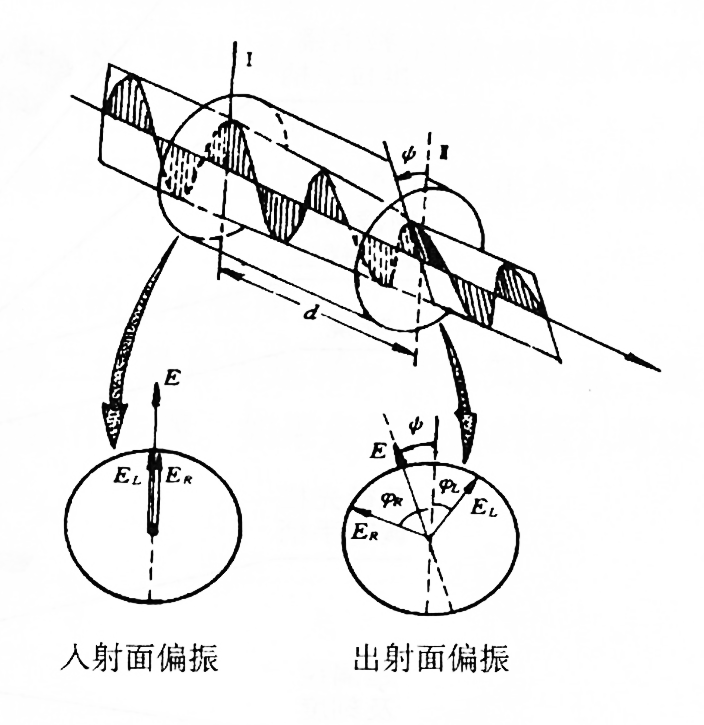
\includegraphics[width=0.6\textwidth]{fig4-1-15}
\caption{旋光性原理示意图}
\label{fig:4-1-15}
\end{figure}
如组成线偏振光的左旋与右旋圆偏光的折射率分别用$n_L$和$n_R$,光波
长用$\lambda$,通过晶体厚度用$d$表示,在两圆偏光自晶片透出的瞬间,二者各具一定周相,二等分其
周相差,就得到离开晶片后的平面偏光的振动方向,此振动方向比原来进入晶片前时的振动方向转动了一
个角度$\Psi$:
\begin{equation}
\Psi=\frac{\phi_L-\phi_R}{2}=\frac{\pi d(n_L-n_R)}{\lambda}.
\end{equation}
由上式可以看出:当$n_L=n_R$时,$\Psi=0$不存在旋光;当$n_L>n_R$时,$\Psi>0$为右旋;当$n_L<n_R$
时,$\Psi<0$为左旋。
当光的波长愈短,晶片的厚度愈大和两圆偏光的双折射率愈大时,偏光面转动的程度
愈大;反之,偏光面的转动愈小。由于两圆偏光的双折射率远较晶体的正常双折射率为小,因此只有在垂直
光轴的切面中且厚度较大时,才能见到较显著的偏光面转动现象。

\section{实验仪器与方法}
\subsection{实验仪器}
\begin{figure}[h!]
\centering
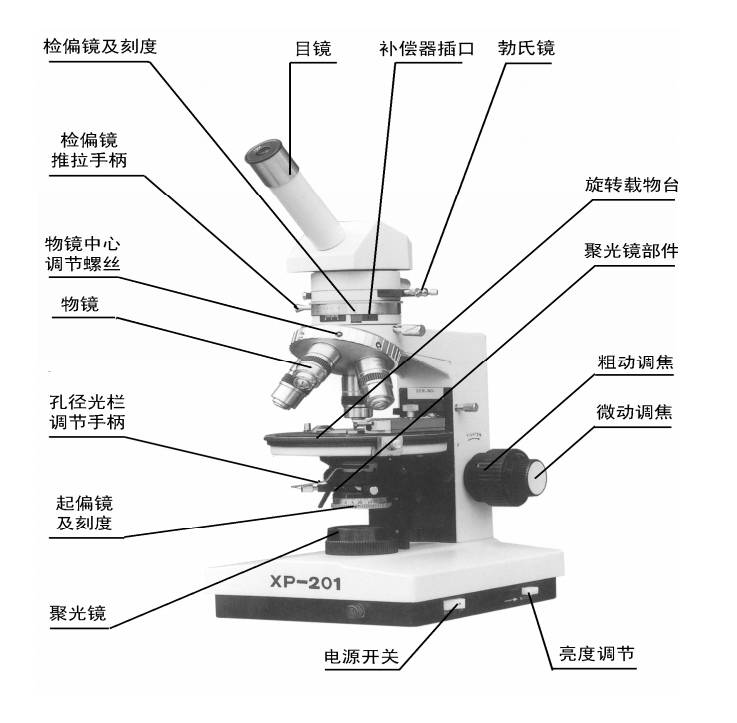
\includegraphics[width=0.7\textwidth]{fig4-1-16}
\caption{$XP-201$型透射偏光显微镜}
\label{fig:4-1-16}
\end{figure}
透射偏光显微种类很多,但基本原理都大同小异。图~\ref{fig:4-1-16}为本实验所用的$XP-201$型透射偏光
显微镜的构造图,主要结构包括:
\begin{enumerate}
\item 光源:卤素灯$12V/20W$,亮度可调节。
\item 起偏镜:用于产生偏振光,可转动调节方向。
\item 聚光镜:位于物台下面,有一组透镜组成,可以把来自下偏光镜的平行光聚敛成锥形偏光,聚光镜连
有手柄,可根据需要旋入或旋出光路。
\item 旋转载物台:用于放置观察样品,可$360$度旋转。
\item 物镜:由四个放大倍数分别我为$4x,10x,40x,60x$的物镜,物镜的前镜片与样品之间的距离称为工作
距离,物镜的工作距离随着放大倍数的增加而减小,所以用高倍物镜时要特别小心,应先将物镜调至最低
,然后逐步升高对焦。
\item 补偿器插口:补偿器插口用于插入各种补偿器,通常仪器带有$\lambda/2,\lambda$及石英楔子等补偿器。
\item 检偏镜:摆动式,可移出光路,进行单偏光观察。
\item 勃氏镜:位于目镜与上偏光镜之间,为一小凸透镜,与目镜联合组成一望远镜,勃氏镜可左右移动
,分别移入、移出光路。
\item 目镜:目镜中装有十字丝和刻度尺。
\end{enumerate}

\subsection{实验方法}
实验给出两组样品:第一组样品的每个晶片都标明了晶体材料及其割面与光轴的大致关系,对第一子样品
的观测可使同学们对于晶体的相关光学性质有一些基本了解和认识;第二组样品都是未知晶片,可供同学
作进一步实际练习和晶体鉴定之用。
\begin{enumerate}
\item 仔细阅读说明书,了解偏光显微镜的结构及使用方法。
\item 校正仪器中心,即调节物镜光轴与物台中心重合。选用低倍物镜,载玻璃片上选一小黑点,并将
小黑点转制十字丝中心,转动载物台,如物镜光轴与载物台中心不重合,小黑点会绕一圆心转动,此圆心
即为载物台中心,调节物镜中心调节螺丝,氏物镜中心移至载物台中心,反复重复调节直至小黑点不在转
动为止。
\item 调整上下偏光镜正交,并使目镜十字丝与上下偏光镜偏振方向平行;在正交偏光镜条件下,将不同
的晶体放在载物台中心,缓缓移动载物台一周,在目镜中仔细观察,准确,完整,简练地描述和记录你所
观察到地原始实验现象。深刻理解什么是全消光,什么是四次消光;并判断给出地几种未知样品是各相同
性质还是各相异性;对已检出地各向异性晶片,用一级红插片判别其慢光方向,并估计其光程差,说明判
别依据。
\item 正交偏光镜成$45$度得位置,然后在试片孔中缓缓插入石英楔子,记录视域中出现得干涉色,查阅
表,根据其色序升降确定样品得慢光振动方向。同理可对斜切和平切片进行上述操作,有余力得同学还可
以对垂直切片进行观测,看看能得出什么结果。
\item 锥光干涉光测:光路中加入锥光镜和勃氏镜,仔细观察晶片得锥光干涉图,然后转动载物台,观测
图形得变化。对各种样品都进行观察和记录,找出这些干涉图得相同点和不同点。有余力的同学,可以换
用高倍物镜重复上述操作,但必须重新校正物镜中心。
\item 鉴定光性正负:依据实验原理所提供得方法,确定所有垂直切片得光性正负。然后开动脑筋,想办法
鉴定斜切样品得光性正负。
\item 利用观察埃利旋转向得方法,判断方和圆两片石英得旋光性质。
\item 选作内容:有时间,有兴趣得同学,还可以从第二组晶片选择一些未知样品,观测其光学性质,
并总结 出快速鉴定样品光学性质得最佳操作步骤。如果条件允许得话,可以观察一下双轴晶体。
\end{enumerate}

\section{实验数据分析}

\section{思考与讨论}
\begin{enumerate}
\item 对于观察者来说,观察消光现象和观察锥光干涉图时,应分别注重观察什么内容?\par 
1)观察消光现象时,应仔细观察四次消光的出现和消光的位置,注重对此现象原理的思考和理解。\par  
2)观察锥光干涉图时,应注意观察锥光图的形态(由一个黑色十字和彩色同心圆构成)和插入石英楔子时
两个形态特征的变化情况,再注重观察各种样品锥光干涉图像的相同点和不同点。\par 
\item 实际观察到的消光现象与你设想的有哪些不同?如何解释?\par 
绝对消光位置并非对应一个严格的角度,而是理论计算的角度加上它的一个很小的邻域,这是由于人的眼睛
对特别微弱的光感觉不到,所以由人眼判断此邻域的光时仍然是暗的。在转动晶体$360^{\circ}$时,观察
到的四明四暗现象只是相对的明、暗。 造成这种情况的原因有以下几个:\par 
1)有外部环境的光线进入观察系统。 \par
2)偏振片的非偏振方向不能完全把光线隔绝,透过的只是近似线偏振光的椭圆偏振光。\par  
3)调节偏振片的时候未能使起偏器和检偏器完全正交。
\item 观察消色时,你看到的颜色可能没有列表中的那么丰富,为什么?此时你应该如何利用消色法则?\par 
在实际观察中,颜色的变化是连续的,而由于视见函数的变化,在紫光波段附近肉眼不敏感,故某些
颜色色带窄,稍微移动晶片颜色就会发生剧烈变化,人眼难以准确分辨。在绿光附近肉眼敏感,图像颜色色
带宽,不同波长的颜色不容易区分。如上述白光干涉的观测可知当光轴与一级红插片的光轴平行时有消光位
置,与一级红插片的光轴成$45^{\circ}$时有最亮位置,而这些位置正是代表了同名轴平行和异名轴平行
以及他们的中间位置的情况,故只需观测这些位置,便可忽略其他的位置及色序。 \par 
考虑到绿色和黄色的色带宽,人眼敏感,色带较宽而人眼判断的主观性很强,对于定出干涉光的波长可能误
差较大,这样估计出的晶片的光程差会有很大的误差。我们可以考虑找一些色带较小的波段,使用该波段对
应的插片,再根据干涉色序表定出其波长,其对应的颜色也较为容易判断。也可以使用频谱探测仪器代替眼
睛,这样能得到十分精确的结果。
\item 向异性的晶片放于正交偏光镜下,当转动载物台一周时,出现四次消光,如何解释?\par 
上下偏振片偏振方向正交,所以不加晶片的时候,视场全暗。当在正交偏光镜之间加入一各相异性晶体时,
一束波长为$\lambda$的光波经正交偏光镜和晶片后,会变成大小相等而振动方向相反,频率相同,位相差
恒定的两束光($o$光和$e$光),它们满足干涉条件,由平面波叠加原理,其合成光强由式~\eqref{eq:4-1-6}
描述
\begin{equation}
I\propto A_+^2= A_{oe}^2\sin^22\alpha\sin^2\big[\frac{d(n_e-n_o)}{\lambda}\pi\big].
\end{equation}
对于单色光,当$\alpha=0,\pi/2,\pi,\ldots$时,$sin2\alpha=0$,即当晶片的轴向与两正交偏光镜其中之一
的偏振方向一致时,合成光强为零,视野全暗,此现象称为消光现象。此时,晶片的位置称为消光位置。当
$\alpha=\pi/4,3\pi/4,5\pi/4,\ldots$时,$sin2\alpha=\pm 1$,即当晶片的轴向处于两个偏光镜的偏振方向
中间时,合成光强最大,视阈最亮。很显然,如转动晶片$360$度,会出现四暗、四明现象。\par
\item 双折射率较低时,黑十字粗些,而双折射率较高或双折射率不太高而晶片较厚时,黑十字较前者细
些, 如何解释?\par 
对于双折射率较低的晶体,要产生相同的光程差就需要通过更长的距离,故对于固定厚度的晶片,光束的干涉
就较少,因此消光影相应的要粗些。同理, 双折射率较高的或双折射率不太高而晶片较厚时,光束的干涉较多,
因此消光影相应的要细些。
\item 平行光轴切片的晶体厚度较大时,沿光轴方向的干涉色是否肯定愈向外愈低,为什么?\par 
不一定。对于强聚敛光情况,对处于光锥外缘的光,可能出现厚度对于光程差的影响超过双折射率对于光程差的影响。
在这种情形下,沿光轴方向,开始时会出现干涉色降低现象,而等到了视域边缘干涉色又会逐渐升高。
\end{enumerate}




%\medskip
%\renewcommand{\refname}{参考文献}
%\begin{thebibliography}{99}
%\bibitem{wiki}Franck–Hertz experiment. Wikipedia[DB/OL]. \url{http://en.wikipedia.org/wiki/Franck%E2%80%93Hertz_experiment}.
%\bibitem{ref01}蔡文. 可拓论及其应用[J]. 科学通报, (1999),44(7), 673-682.
%\bibitem{data}Hg (all spectra). NIST Atomic Spectra Database Lines Data[DB/OL]. \url{http://physics.nist.gov/cgi-bin/ASD/lines1.pl}.
%\bibitem{ref03}杨福家. 原子物理学[M]. 高等教育出版社,北京. 2008.
%\bibitem{reffh}Rapior, G.; Senstock, K.; Baev, V.. New features of the Franck–Hertz experiment[J]. Amer. J. Phys. (2006), 74: 423–428.
%\bibitem{ref03}Warren J. Smith. Modern Optical Engineering[M]. McGraw-Hill Education,New York. 2007.
%\bibitem{ref04}曹炳元. 物元分析法及其在投资决策中的应用[C]. 中国第二次物元分析学术讨论会论文选. 广州, 1986.
%\end{thebibliography}
\end{CJK*}
%\begin{CJK*}{UTF8}{gbsn}
%\newpage
%\renewcommand{\appendixname}{附录}
%%\appendix
%\begin{appendices}
%  \renewcommand\thetable{\thesection\arabic{table}}
%  \renewcommand\thefigure{\thesection\arabic{figure}}
%  \section{电子自旋共振实验}
%  日期:2015.10.13 \hfill{} 室温:25.0$^\circ C$ \hfill{}湿度:75.0\% \hfill{}实验人:胡乃超 \ 金谷柳新
%  \section{实验过程记录} \label{app:foobar}
%
%\end{appendices}
%\end{CJK*}
\end{spacing}
\end{document}
